\begin{figure}[]
     \centering
     \begin{subfigure}[b]{0.48\textwidth}
         \centering
         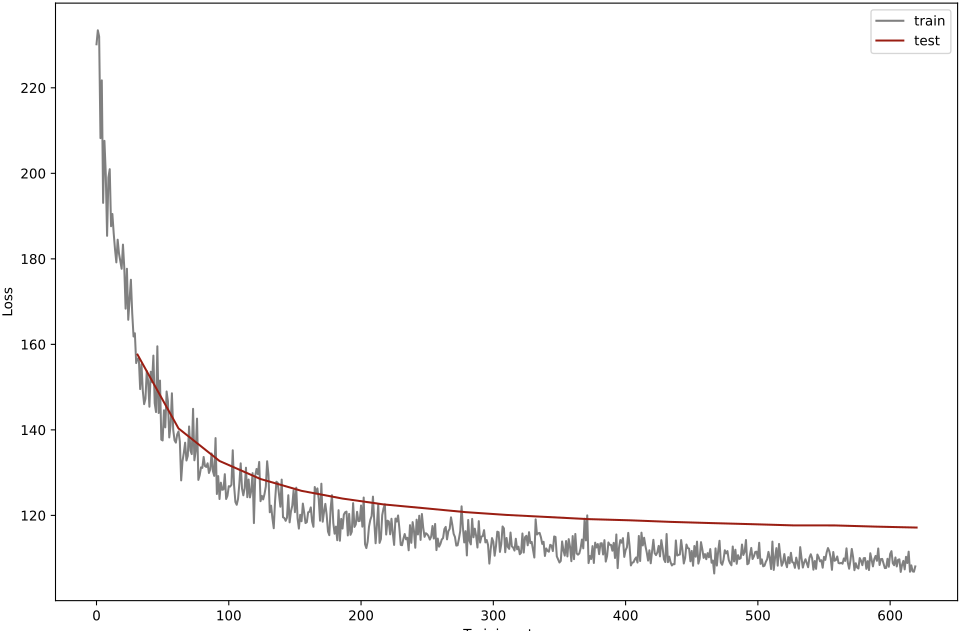
\includegraphics[width=\textwidth]{observational/img/bnn/mc/LC_mc1e-10.png}
         \caption{Loss; $mc=0$}
     \end{subfigure}
     \hfill
     \begin{subfigure}[b]{0.48\textwidth}
         \centering
         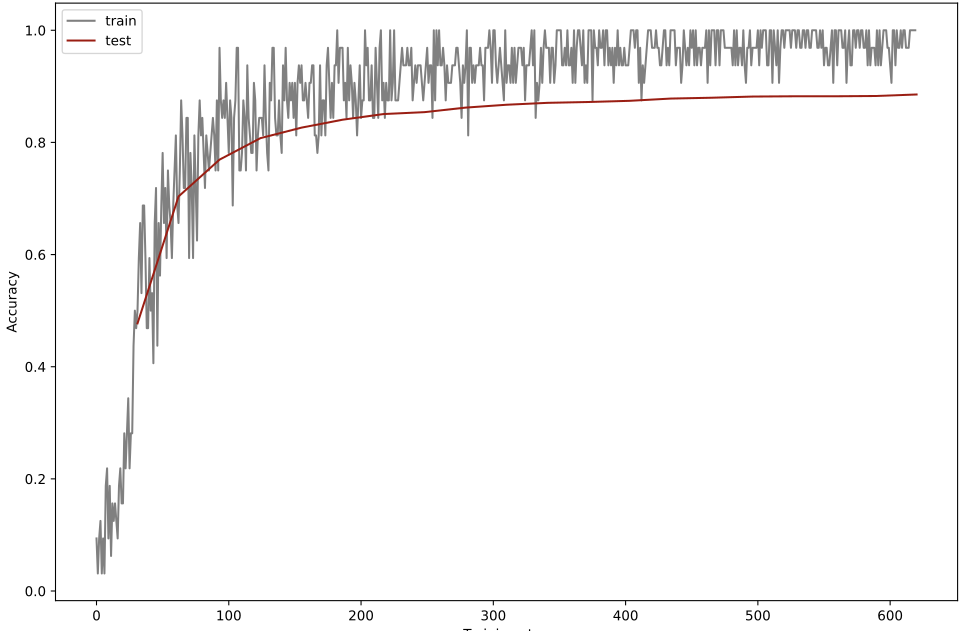
\includegraphics[width=\textwidth]{observational/img/bnn/mc/AC_mc1e-10.png}
         \caption{Accuracy; $mc=0$}
     \end{subfigure}
     \caption[Mixing coefficient values influence on the BNN learning process]{Mixing coefficient values influence on the Bayesian Neural Network learning process.}
    \label{fig:bnn-mc}
\end{figure}
\begin{figure}[]\ContinuedFloat
     \begin{subfigure}[b]{0.48\textwidth}
         \centering
         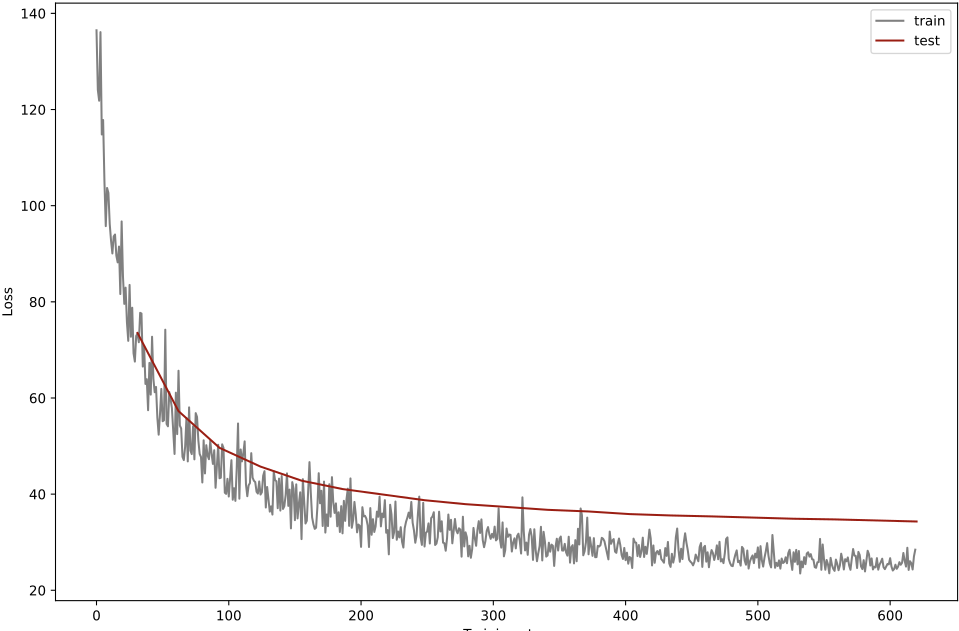
\includegraphics[width=\textwidth]{observational/img/bnn/mc/LC_mc0.1.png}
         \caption{Loss; $mc=0.1$}
     \end{subfigure}
     \hfill
     \begin{subfigure}[b]{0.48\textwidth}
         \centering
         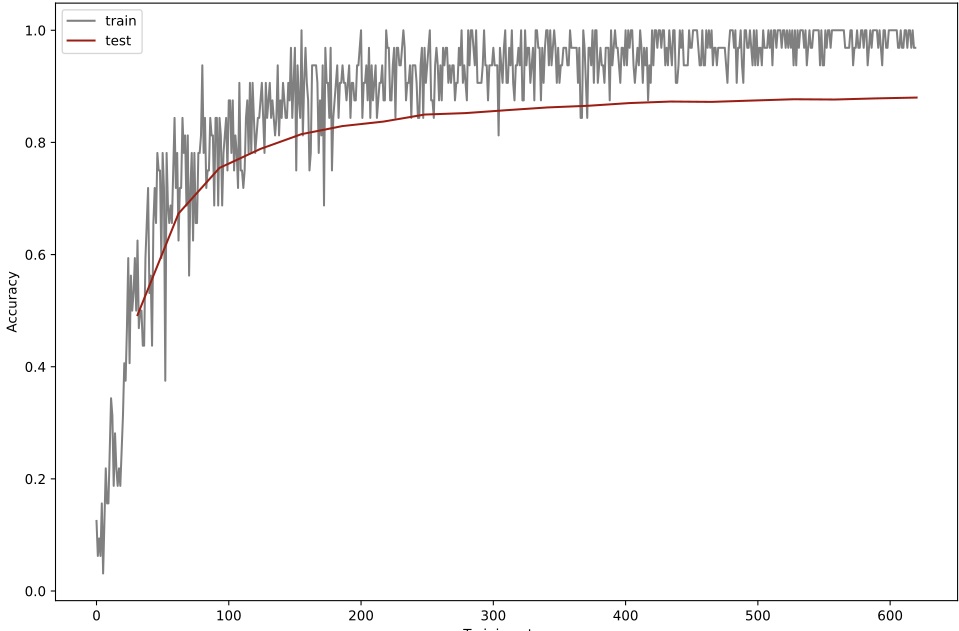
\includegraphics[width=\textwidth]{observational/img/bnn/mc/AC_mc0.1.png}
         \caption{Accuracy; $mc=0.1$}
     \end{subfigure} 
     \par\bigskip
     \begin{subfigure}[b]{0.48\textwidth}
         \centering
         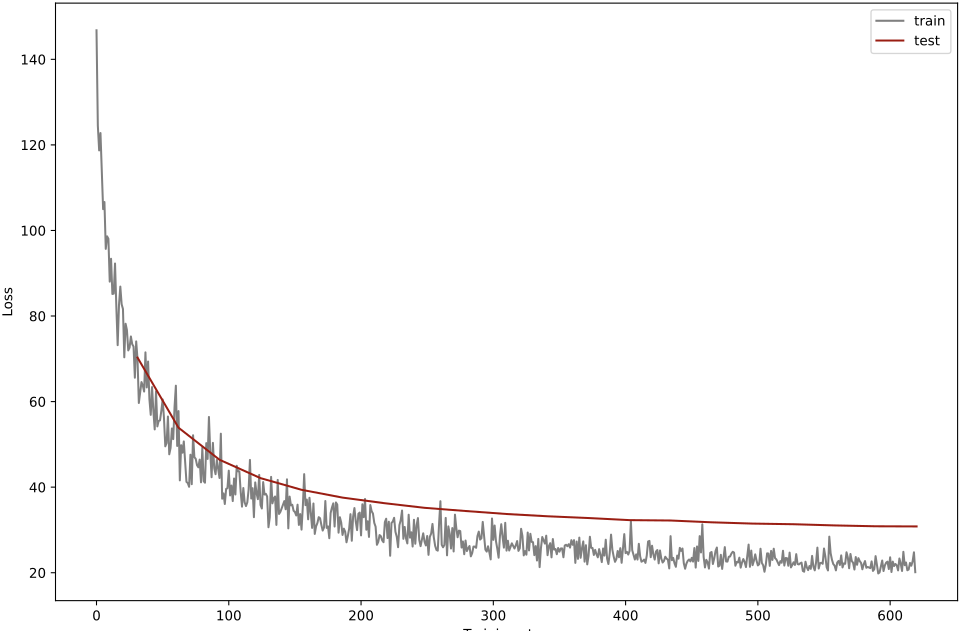
\includegraphics[width=\textwidth]{observational/img/bnn/mc/LC_mc0.25.png}
         \caption{Loss; $mc=0.25$}
     \end{subfigure}
     \hfill
     \begin{subfigure}[b]{0.48\textwidth}
         \centering
         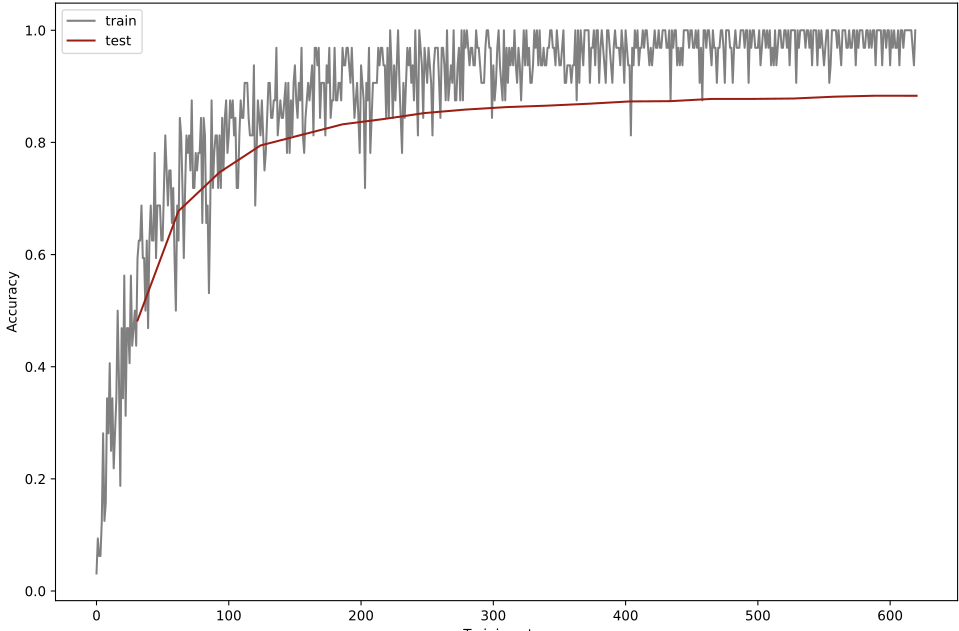
\includegraphics[width=\textwidth]{observational/img/bnn/mc/AC_mc0.25.png}
         \caption{Accuracy; $mc=0.25$}
     \end{subfigure} 
     \par\bigskip
     \begin{subfigure}[b]{0.48\textwidth}
         \centering
         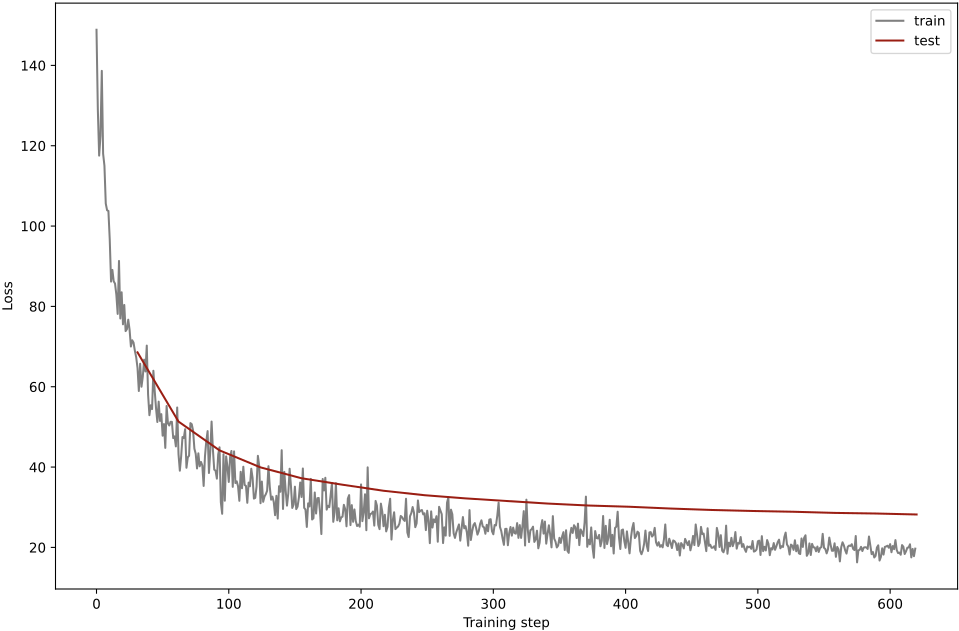
\includegraphics[width=\textwidth]{observational/img/bnn/mc/LC_default.png}
         \caption{Loss; $mc=0.5$}
     \end{subfigure}
     \hfill
     \begin{subfigure}[b]{0.48\textwidth}
         \centering
         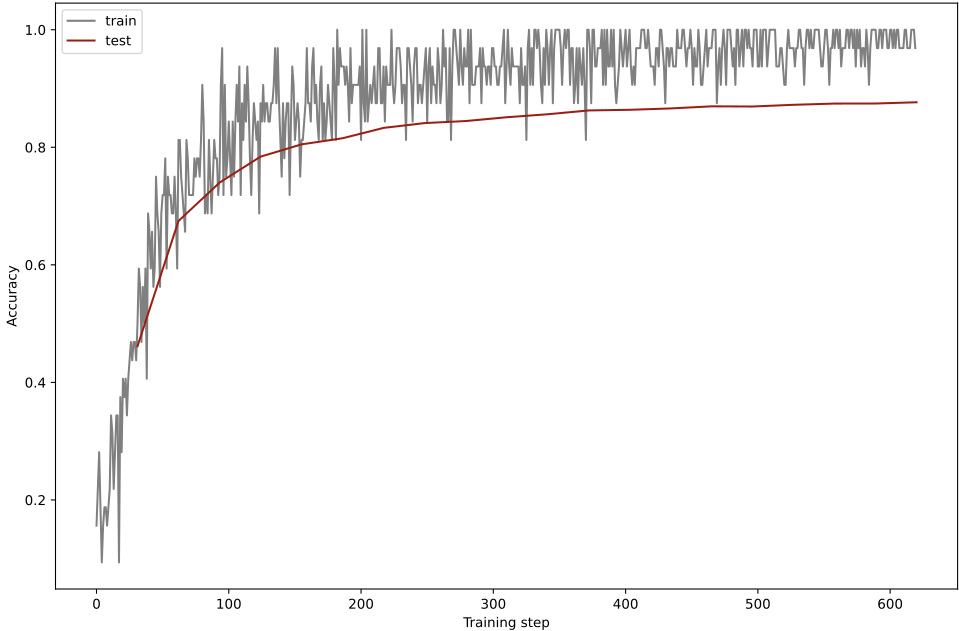
\includegraphics[width=\textwidth]{observational/img/bnn/mc/AC_default.png}
         \caption{Accuracy; $mc=0.5$}
     \end{subfigure} 
     \caption[]{Mixing coefficient values influence on the Bayesian Neural Network learning process (cont.).}
\end{figure}
\begin{figure}[]\ContinuedFloat
     \begin{subfigure}[b]{0.48\textwidth}
         \centering
         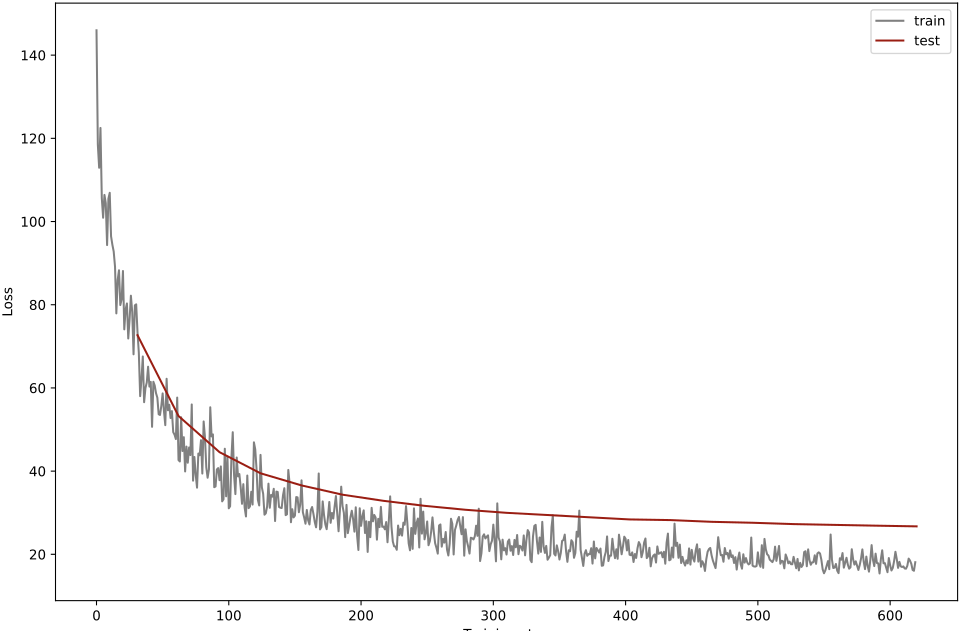
\includegraphics[width=\textwidth]{observational/img/bnn/mc/LC_mc0.75.png}
         \caption{Loss; $mc=0.75$}
     \end{subfigure}
     \hfill
     \begin{subfigure}[b]{0.48\textwidth}
         \centering
         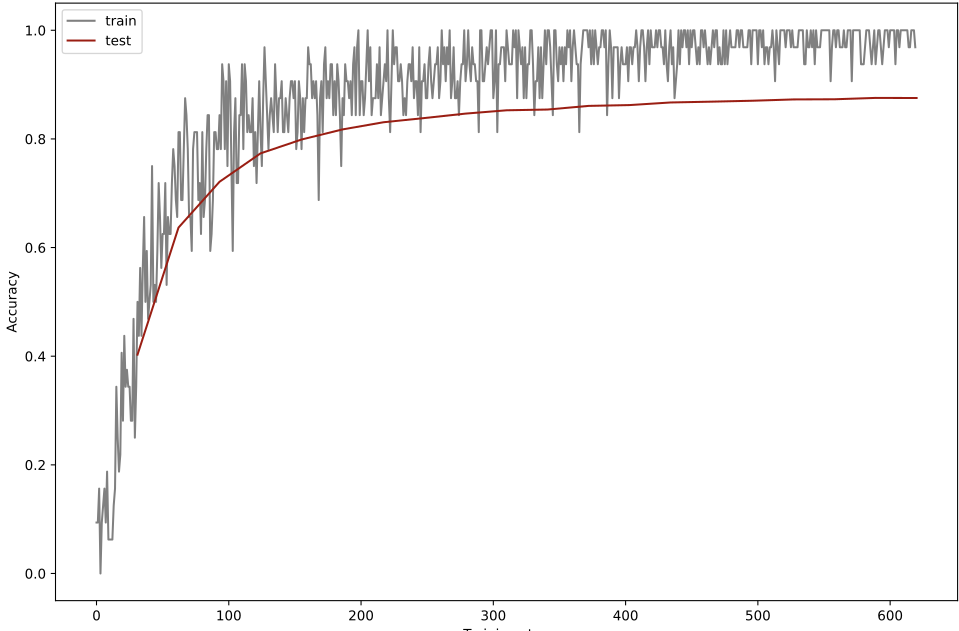
\includegraphics[width=\textwidth]{observational/img/bnn/mc/AC_mc0.75.png}
         \caption{Accuracy; $mc=0.75$}
     \end{subfigure} 
     \par\bigskip
     \begin{subfigure}[b]{0.48\textwidth}
         \centering
         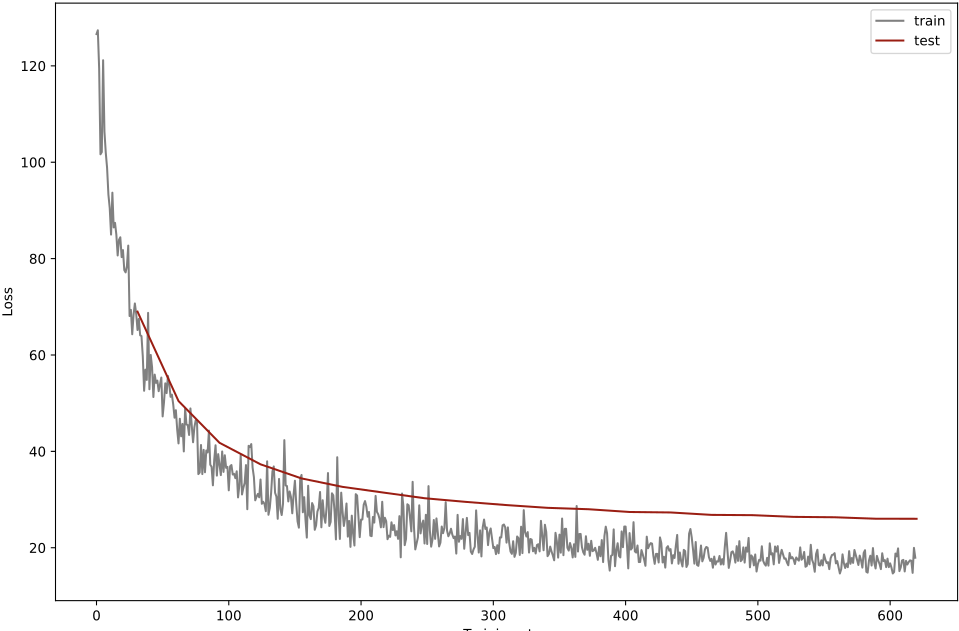
\includegraphics[width=\textwidth]{observational/img/bnn/mc/LC_mc0.9.png}
         \caption{Loss; $mc=0.9$}
     \end{subfigure}
     \hfill
     \begin{subfigure}[b]{0.48\textwidth}
         \centering
         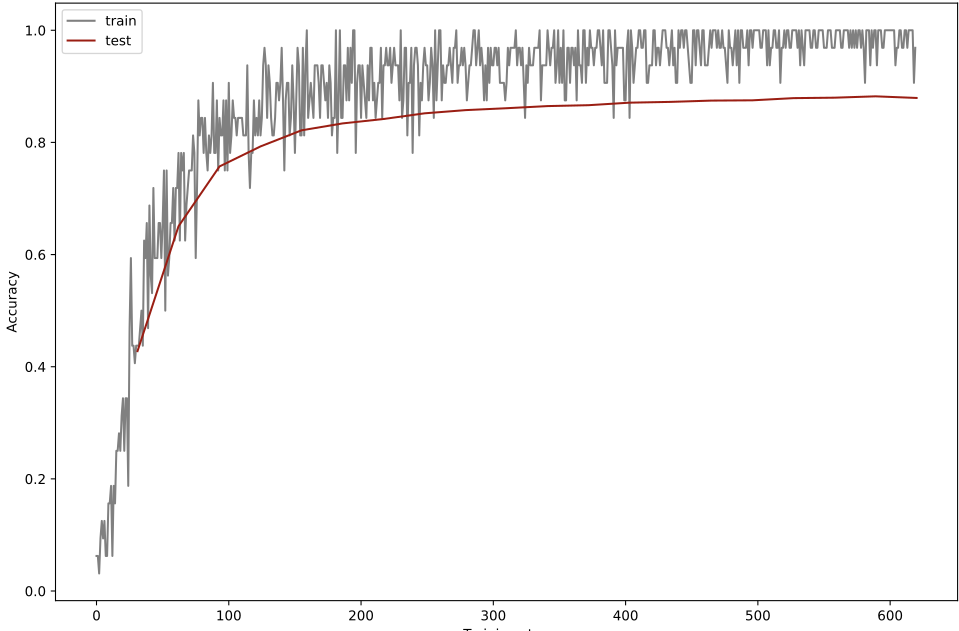
\includegraphics[width=\textwidth]{observational/img/bnn/mc/AC_mc0.9.png}
         \caption{Accuracy; $mc=0.9$}
     \end{subfigure} 
     \par\bigskip
     \begin{subfigure}[b]{0.48\textwidth}
         \centering
         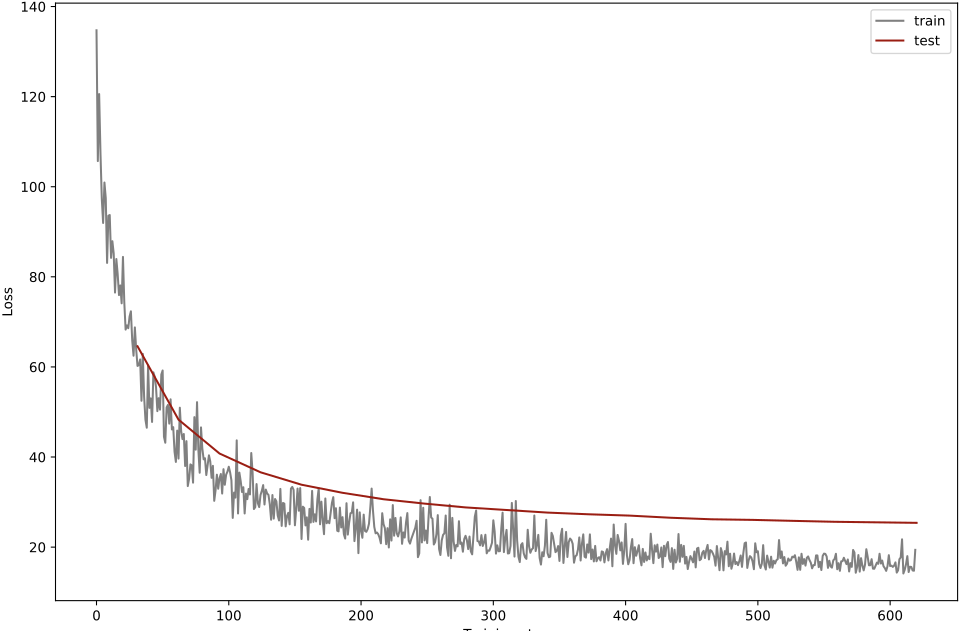
\includegraphics[width=\textwidth]{observational/img/bnn/mc/LC_mc1.png}
         \caption{Loss; $mc=1$}
     \end{subfigure}
     \hfill
     \begin{subfigure}[b]{0.48\textwidth}
         \centering
         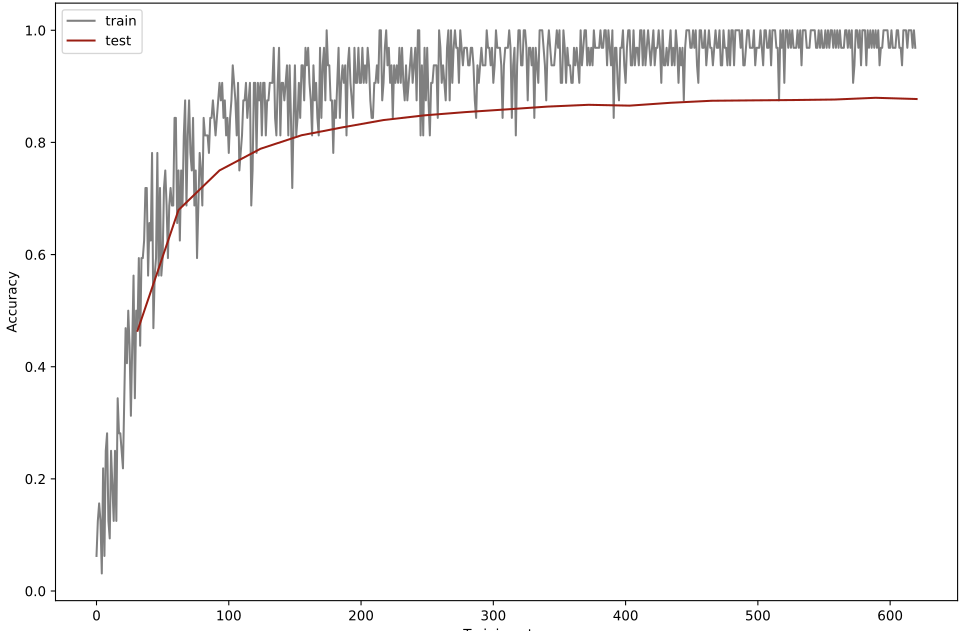
\includegraphics[width=\textwidth]{observational/img/bnn/mc/AC_mc1.png}
         \caption{Accuracy; $mc=1$}
     \end{subfigure} 
     \caption[]{Mixing coefficient values influence on the Bayesian Neural Network learning process (cont.).}
\end{figure}